\section{Introduction}

\subsection{Outline}
\begin{frame}{Lecture 3: Statistical Inference}
  \begin{itemize}
    \item In the last lecture, we described {\bf descriptive statistics}, such as point and interval estimators.\bigskip

    \item Point and interval estimators are very useful to define the value of parameters in the population, and to estimate their margins of errors.\bigskip

    \item However, in some cases, we need {\bf decision making tools}, in order to deal with information from random samples.\bigskip

    \item {\bf Statistical Inference} is one of these tools that can help us \structure{make a decision based on a random sample}.
  \end{itemize}
\end{frame}

\begin{frame}{Statistical Inference}{Motivating Example}

  \begin{columns}
    \column{.8\textwidth}
    Imagine you are the owner of a factory that produces delicious chocolate. Its packages should contain \structure{300g of chocolate}.
    \column{.2\textwidth}
    \hfill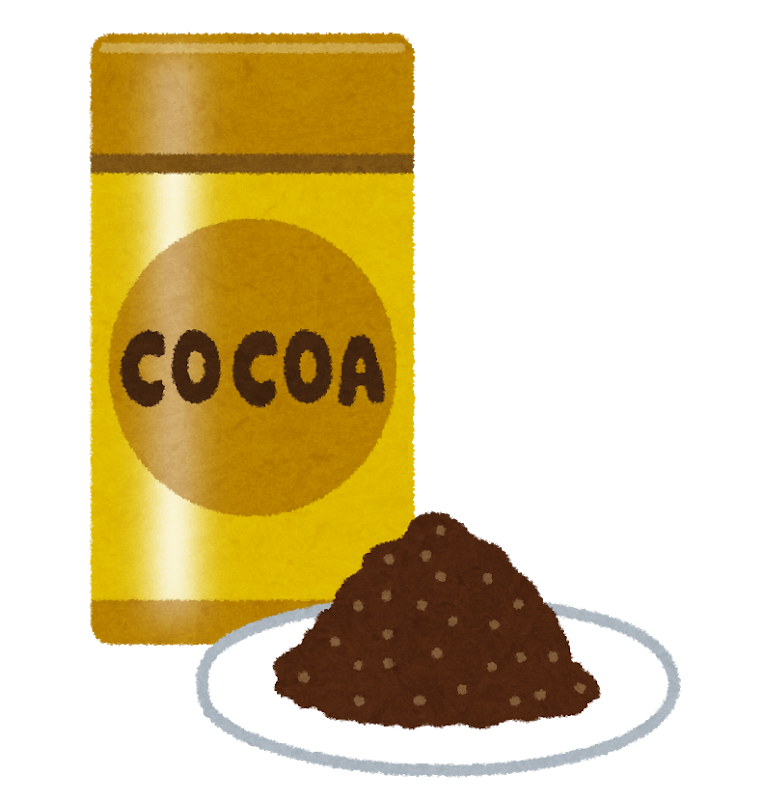
\includegraphics[width=1\textwidth]{../img/irasutoya_cocoa}
    \ppagenote{Cocoa image from \url{https://www.irasutoya.com}}
  \end{columns}

  You take a sample of {\bf 30 packages} produced by your factory. Using the tools from lecture 2, you calculate the mean weight with a 95\% confidence interval of {\bf 283g to 307g}.\bigskip

  Is everything normal? Or should you investigate the production line of your factory?\bigskip

  \begin{alertblock}{Remember!}
    The confidence interval does not say whether {\bf any of the values inside it} are more or less likely than any other!
  \end{alertblock}
\end{frame}


\subsection{Scientist}
\begin{frame}{Florence Nightingale}{1820-1910 -- "The Lady with the Lamp"}
  \begin{columns}
    \column{.3\textwidth}
      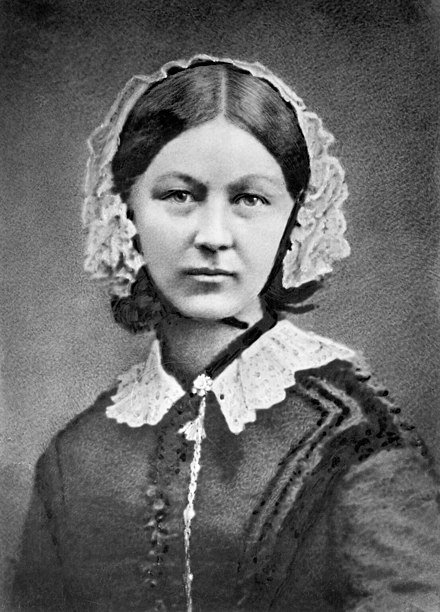
\includegraphics[width=\textwidth]{../img/florence}
    \column{.7\textwidth}
      Let's talk about a scientist who made great contributions to evidence-based medicine and descriptive statistics: {\bf Florence Nightingale}.\bigskip

      \begin{itemize}
        \item British nurse and mathematician;\medskip

        \item Born in 05/12/1820, her parents were opposed to her careers;
        \item She was driven, a prolific writer, and knew several languages;
        \medskip

        \item Gave great contributions for the professionalization of nursing;
      \end{itemize}
  \end{columns}
\end{frame}

\begin{frame}{Florence Nightingale}{Descriptive Statistics in Health}
  \begin{itemize}
    \item Implemented the use of {\bf hand washing} in hospitals for nurses:
    \item Pioneer of using of data visualization (infographics!) in medicine;
  \end{itemize}
  \begin{center}


    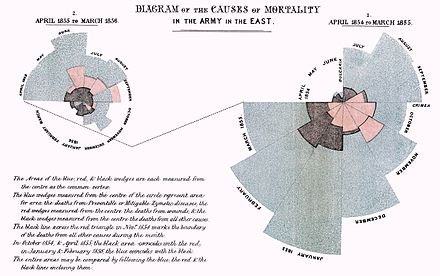
\includegraphics[width=.7\textwidth]{../img/florence_diagram}
  \end{center}
\end{frame}

\subsection{Fair Comparisons}
% - Fair Comparisons:

\begin{frame}{Experiment Design: Fair Comparisons}{A sombering example}

  Musgrave et al (preprint): several ML methods for metric learning perform exaclty the same when the hyperparameters are properly tuned for all methods.

  \begin{center}
    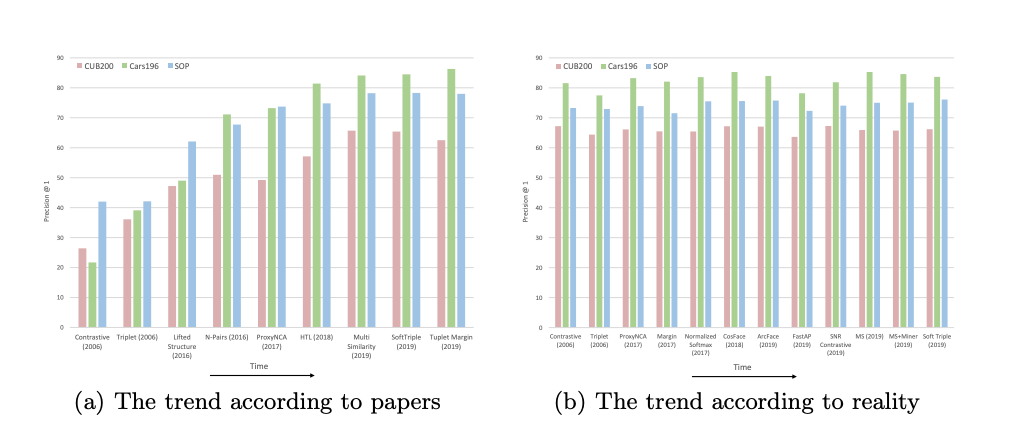
\includegraphics[width=.8\textwidth]{../img/musgrave_faircomparison}\\
    {\tiny Figure from Musgrave et al. "A Metric Learning Reality Check"}
    \ppagenote{Figure from Musgrave et al. "A Metric Learning Reality Check" \url{https://arxiv.org/pdf/2003.08505.pdf}}
  \end{center}

  \alert{Fair comparisons will help you avoid false conclusions!}
\end{frame}

\begin{frame}{Experiment Design: Fair Comparisons}{What are fair comparisons?}
  The definition of a {\bf fair} comparison, of course, depends on the field being studied and the experiment being conducted. In the comparison of algorithms in computer science, we can think of some points:
  \begin{itemize}
    \item Fine-tuning of algorithmic parameters;
    \item Discarding failed variations;\medskip
    \item Fine-tuning of the algorithm itself on the training data;
    \item Only comparing on data favorable to one of the algorithms;\medskip
    \item Coding with modern libraries vs old algorithms;
    \item Different computational environments;
    \item etc...
  \end{itemize}
\end{frame}

\begin{frame}{Lecture 3: Outline}
  \begin{itemize}
    \item What is Statistical Inference?\bigskip
    \item Statistical Hypothesis and Errors;\bigskip
    \item Z testing on a single sample;\bigskip
    \item Statistical Testing Assumptions;\bigskip
  \end{itemize}
\end{frame}
